\begin{boiboiboite}
	\propeau
	\propair
	\isentropiques
	\deltaentropie
\end{boiboiboite}

% ajouter un exo proposant de tracer les diagrammes T-s pour les moteurs étudiés dans d’autres chapitres

\subsubsection{Détente d’un liquide/vapeur}

	Une masse de~\SI{10}{\kilogram} d’eau est à~\SI{45}{\bar} et~\SI{600}{\degreeCelsius}.
	
	\begin{enumerate}
		\item Quelle est la quantité maximale de travail qu’il est possible d’extraire de cette masse d’eau, sans lui fournir de chaleur, si on peut la détendre jusqu’à~\SI{4}{\bar} ?
		\item Si la détente était poursuivie jusqu’à une pression plus basse, à quelle température l’eau se condenserait-elle ?
		\item Représentez l’évolution sur un diagramme température-entropie, de façon qualitative (c’est-à-dire sans représenter les valeurs numériques), et en y représentant la courbe de saturation.
	\end{enumerate}

\subsubsection{Variations élémentaires d’un gaz parfait}

	Parmi les évolutions d’un gaz parfait décrites en \cref{fig_tsel}, identifiez l’évolution à température constante, à pression constante, isentropique, et à volume constant.	
	
	\begin{figure}
		\begin{center}
			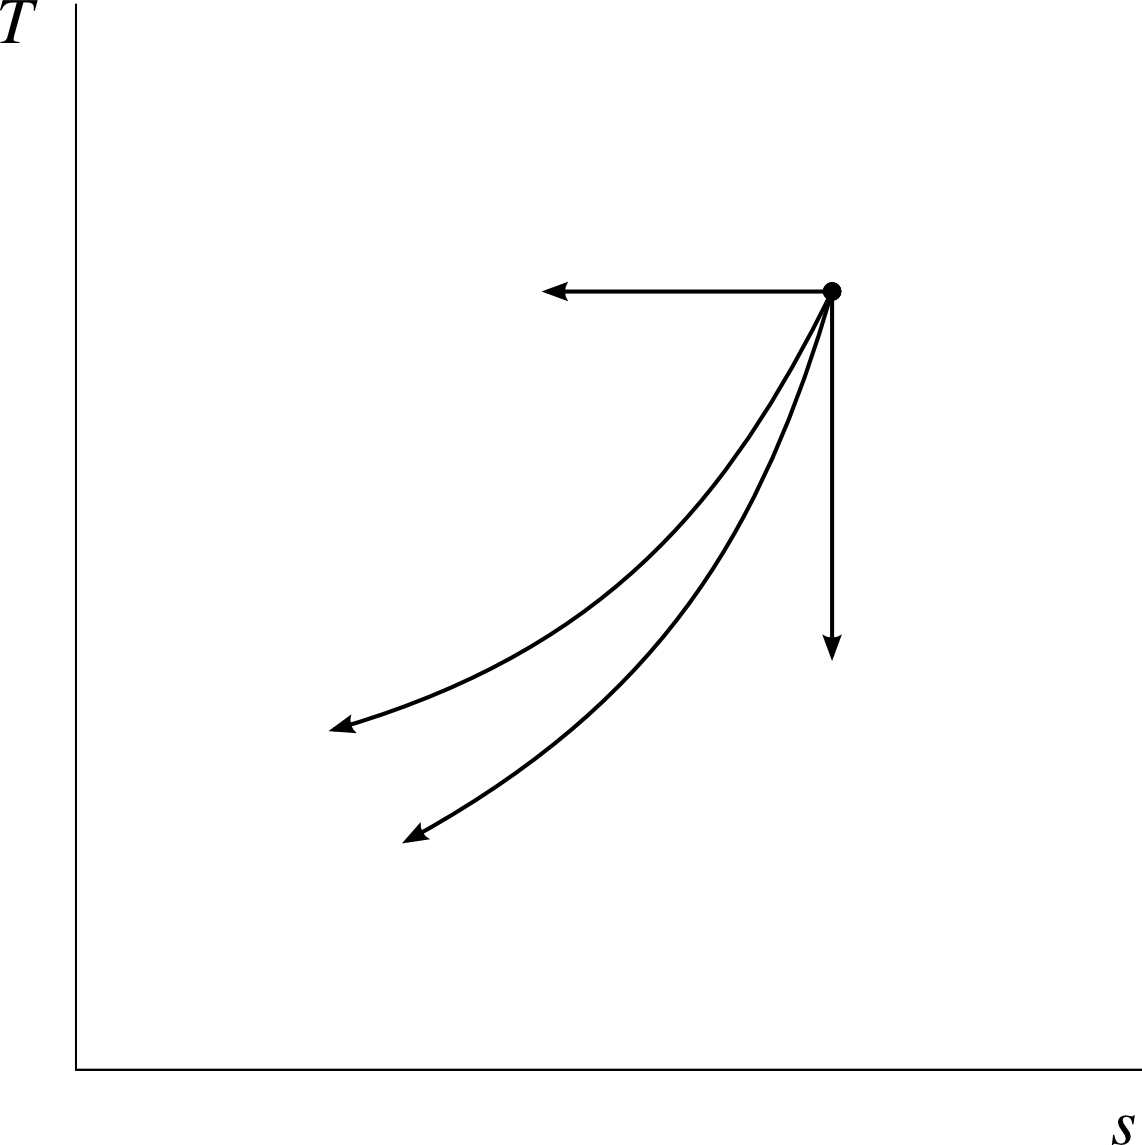
\includegraphics[width=7cm]{images/tsel1.png}
			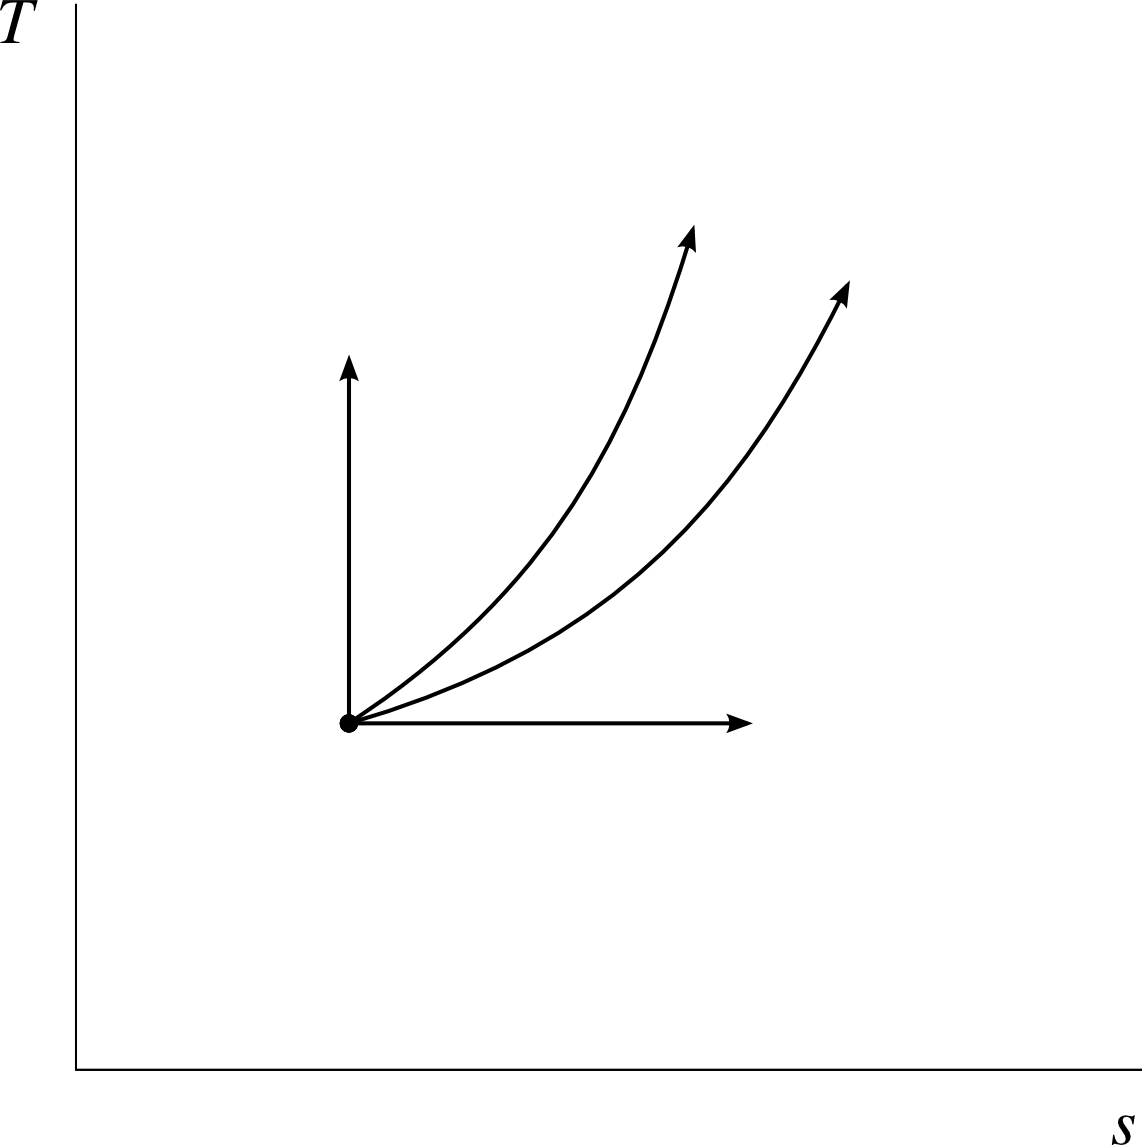
\includegraphics[width=7cm]{images/tsel2.png}
		\end{center}
		\caption{Évolutions élémentaires d’un gaz parfait}
		\label{fig_tsel}
	\end{figure}


\subsubsection{Chauffage à température constante}

	On fournit lentement une quantité de chaleur \SI{3000}{\kilo\joule\per\kilogram} à une masse d’eau liquide saturée à~\SI{200}{\degreeCelsius}. La température est maintenue constante pendant toute l’évolution.
	
	Quelle est la quantité de travail développée par l’eau pendant l’évolution ? Représentez l’évolution sur un diagramme pression-volume, de façon qualitative et en y représentant la courbe de saturation.
	
\subsubsection{Cycle de Carnot}

	Représentez le cycle suivi par le fluide à l’intérieur d’une pompe à chaleur opérant selon le cycle de Carnot sur un diagramme pression-volume, de façon qualitative, et en y représentant les deux transferts de chaleur.
	
	Comment le cycle serait-il modifié si la compression et la détente restaient adiabatiques mais n’étaient pas réversibles ?

\subsubsection{Turbine à vapeur}

	Dans une centrale à vapeur, un débit de~\SI{250}{\tonne\per\hour} de vapeur rentre à~\SI{55}{\bar} et~\SI{660}{\degreeCelsius} dans la turbine.
	
	La turbine détend la vapeur de façon adiabatique réversible. Lorsque la pression atteint \SI{10}{\bar}, on prélève de la vapeur avec un faible débit (\SI{1}{\kilogram\per\second}), pour réchauffer une autre partie de la centrale. La vapeur restant dans la turbine est détendue jusqu’à une pression de~\SI{0,18}{\bar}.
	
	Quelle est la puissance mécanique développée par la turbine ?

\subsubsection{Sens des transformations (1)}

	Une masse d’air suit une évolution sans apport de chaleur. Il y a deux états :
		\begin{itemize}
			\item Un état $X$ à~\SI{5}{\bar} et~\SI{500}{\degreeCelsius} ;
			\item Un état $Y$ à~\SI{1}{\bar} et~\SI{300}{\degreeCelsius}.
		\end{itemize}
		
	Quel est le seul sens ($X \to Y$ ou $Y \to X$) dans lequel l’évolution peut avoir lieu ?
	
	Représentez l’évolution sur un diagramme pression-volume et sur un diagramme température-entropie, de façon qualitative.

\subsubsection{Sens des transformations (2)}

	De l’eau suit une évolution pendant laquelle on lui retire \SI{2}{\mega\joule\per\kilogram} de chaleur (sa température étant alors figée à~\SI{250}{\degreeCelsius}). Il y a deux états, un au début et l’autre à la fin :
		\begin{itemize}
			\item Un état $X$ à l’état de vapeur saturée à~\SI{200}{\degreeCelsius} ;
			\item Un état $Y$ à l’état de liquide saturé à~\SI{240}{\degreeCelsius}.
		\end{itemize}
	Quel est le seul sens ($X \to Y$ ou $Y \to X$) dans lequel l’évolution peut avoir lieu ?

\subsubsection{Détente d’air comprimé}

	L’air dans un cylindre isolé thermiquement est détendu depuis \SI{6,8}{\bar} et~\SI{430}{\degreeCelsius} jusqu’à~\SI{1}{\bar}.

	À la sortie, la température est mesurée à~\SI{150}{\degreeCelsius}.

	La détente est-elle réversible ? Représentez l’évolution sur un diagramme température-entropie, de façon qualitative.

\subsubsection{Questions de cours}

	\begin{enumerate}
		\item Quelle est la différence entre l’entropie et la capacité calorifique, qui ont toutes les deux les mêmes unités ?
		\item À quoi ressemblerait la \cref{fig_expérience_création_entropie_t-s} si le transfert de chaleur était poursuivi au-delà d’une quantité infinitésimale de chaleur $\diff Q$ ?
	\end{enumerate}


\subsubsection{Pompe à air}

	De l’air rentre dans une petite pompe centrifuge avec un débit de~\SI{4}{\kilogram\per\minute}. La pompe n’est pas isentropique, mais on peut négliger ses pertes de chaleur. 

	À l’entrée, l’air est  à~\SI{1}{\bar} bar et~\SI{15}{\degreeCelsius}.\\
	À la sortie, la pression est à~\SI{2}{\bar} et on mesure la température à~\SI{97}{\degreeCelsius}.

	\begin{enumerate}
		\item Quelle est la puissance requise pour alimenter le compresseur ?
		\item Quelle serait la puissance si la compression se faisait de façon isentropique ?
		\item Quels seraient les transferts de chaleur et de travail nécessaires pour ramener l’air à ses conditions initiales (en minimisant les transferts de chaleur) ?
	\end{enumerate}

\subsubsection{Centrale électrique théorique}
	
	Pendant la conception d’une centrale électrique on étudie la possibilité de faire suivre à l’eau un cycle de Carnot. La chaleur dégagée par la combustion du charbon est transmise à une chaudière à vapeur. La vapeur est détendue dans une turbine, qui alimente une génératrice électrique. 

	\begin{description}
		\item[De A à B] L’eau est compressée dans une pompe isentropique.\\
			En A, le mélange liquide-vapeur est à pression de~\SI{0,04}{\bar}.\\
			En B, l’eau est à l’état de liquide saturé, à pression de~\SI{40}{\bar}.
		\item[De B à C] L’eau est chauffée à pression constante (\SI{40}{\bar}) dans la chaudière. 
			En C, l’eau est à l’état de vapeur saturée.
		\item[De C à D] L’eau est détendue dans la turbine isentropique. 
			En D, l’eau est à la pression initiale, c’est-à-dire \SI{0,04}{\bar}.
		\item[De D à A] L’eau est refroidie dans un condenseur à pression constante (\SI{0,04} bar).
	\end{description}

\begin{enumerate}
	\item Schématisez les éléments du circuit suivi par la vapeur, et représentez l’évolution sur un diagramme température-entropie, de façon qualitative et en y représentant la courbe de saturation.
	\item Quel est le titre de l’eau lorsque la condensation est interrompue (en A) ? Quelle est alors l’enthalpie spécifique ?
	\item Quel est le titre à la sortie de la turbine (en D) et l’enthalpie spécifique en ce point ?
	\item Quelle est la puissance développée par la turbine ?
	\item Quelle est la puissance de la chaudière ?
	\item Quelle est la puissance de la pompe ?
	\item Quel est le rendement de l’installation ?
\end{enumerate}

\subsubsection{Transferts de chaleur irréversibles}

	Un moteur à vapeur fonctionne sur un cycle de Carnot, avec un flux continu (débit :~\SI{2}{\kilogram\per\second}), entre les points de saturation de l’eau. Le moteur est conçu pour exploiter une source de chaleur à moyenne température (\SI{400}{\degreeCelsius}), issue de la combustion de déchets industriels, et rejeter de la chaleur dans une rivière à basse température (\SI{10}{\degreeCelsius}).

	La chaudière a des parois épaisses pour réduire l’impact des imperfections de fabrication et pour soutenir la pression élevée de l’eau. Cette épaisseur impose un gradient de température important à travers les parois (\SI{10}{\degreeCelsius}). Il en va de même dans le condenseur (gradient :~\SI{5}{\degreeCelsius} de gradient).

	\begin{enumerate}
		\item De combien l’entropie de l’ensemble \{source de chaleur + eau\} augmente-t-elle ?
		\item De combien l’entropie de l’ensemble \{puits de chaleur + eau\} augmente-t-elle ?
		\item Quelle est la perte de puissance associée à cette augmentation d’entropie ?
		\item Quelle(s) propriété(s) du matériau constituant la chaudière sont-elles les plus désirables pour minimiser ce problème ?
	\end{enumerate}


\subsubsection{Compressions et détentes irréversibles}

	L’équipe d’ingénieurs en charge du moteur de l’exercice précédent (cycle de Carnot fonctionnant entre \SI{290}{\degreeCelsius} et~\SI{15}{\degreeCelsius}) découvre que les phases de compression et détente ne se font pas de façon réversible.

	Le compresseur amène bien l’eau à température haute mais sa consommation de travail est \SI{10}{\percent} plus importante que prévu. La turbine amène bien l’eau à température basse, mais elle fournit \SI{10}{\percent}  d’énergie mécanique en moins que prévu.
	
	\begin{enumerate}
		\item De combien l’entropie de la vapeur augmente-t-elle dans chacun de ces deux composants ?
		\item De combien augmentent les rejets de chaleur ?
		\item Quelle est la perte en efficacité de l’installation par rapport à une installation réversible ?
	\end{enumerate}


\exercisesolutionpage
\titreresultats
	\linktosolutionsblurb

	\begin{description}
		\item [8.1] \tab 1) $u_1 = \SI{3276,4}{\kilo\joule\per\kilogram} $ et $u_1 = \SI{2703,3}{\kilo\joule\per\kilogram}$ : $W_\text{max.} = \SI{-5,731}{\mega\joule}$. 
						\tab 2) $T_3 = \SI{103,51}{\degreeCelsius}$
		\item [8.2] \tab \textit{Dans le sens horaire, en partant de la verticale, sur les deux graphiques :} isentropique, isochore, isobare, isotherme.
		\item [8.3] \tab $s_2 = \SI{8,671}{\kilo\joule\per\kelvin\per\kilogram}$ ; ainsi $u_2 = \SI{2660,89}{\kilo\joule\per\kilogram}$ ; enfin $w_{1\to 2} = \SI{-1,19}{\mega\joule\per\kilogram}$.
		\item [8.5] \tab $h_1 = \SI{3803,5}{\kilo\joule\per\kilogram}$ ; $h_2 = \SI{2677,7}{\kilo\joule\per\kilogram}$ ; $h_3 = \SI{2413,6}{\kilo\joule\per\kilogram}$ : on a donc $\dot{W}_\text{turbine} = \SI{-96,26}{\mega\watt}$.
		\item [8.6] \tab $s_Y - s_X = \SI{+161,08}{\joule\per\kelvin\per\kilogram}$ ainsi le sens est $X\to Y$.
		\item [8.7] \tab On suppose $X\to Y$, alors $\Delta s = \SI{-3,728}{\kilo\joule\per\kelvin\per\kilogram}$ mais $\int_X^Y \left(\frac{\diff q}{T}\right)_\text{chemin réel} = \SI{-3,823}{\kilo\joule\per\kelvin\per\kilogram}$ ainsi le sens est bien $X\to Y$ (encore!).
		\item [8.8] \tab $\Delta s = \SI{+39,77}{\joule\per\kelvin\per\kilogram}$ mais $\int_1^2 \left(\frac{\diff q}{T}\right)_\text{chemin réel} = \SI{0}{\kilo\joule\per\kelvin\per\kilogram}$, ainsi la transformation est irréversible.
		\item [8.10] 	\tab 1) $\dot{W}_\text{pompe} = \SI{+5,493}{\kilo\watt}$
							\tab 2) $\dot{W}_\text{idéal} = \SI{+4,231}{\kilo\watt}$
							\tab 3) Détente lente pour obtenir $\dot{W}_{2\to 1} = \SI{-4,231}{\kilo\watt}$ en refroidissant avec $\dot{Q}_{2\to 1} = \SI{-1,262}{\kilo\watt}$.
		\item [8.12] 	\tab 1) $\dot{S}_\text{haute température} = \SI{+91,77}{\watt\per\kelvin}$ (ou \si[per-mode = symbol]{\joule\per\kelvin\per\second})
							\tab 2) $\dot{S}_\text{basse\ température} = \SI{+92,4}{\watt\per\kelvin}$
							\tab 3) $\dot{W}_\text{perdue} = \SI{+52,14}{\kilo\watt}$
		\item [8.13] 	\tab 1) $\Delta s_\text{compresseur} = \SI{+1,454}{\kilo\joule\per\kelvin\per\kilogram}$ ; $\Delta s_\text{turbine} = \SI{+0,382}{\kilo\joule\per\kelvin\per\kilogram}$
							\tab 2) \SI{+14,6}{\percent}
							\tab 3) \SI{-9}{pt} (jusqu’à~\SI{39,82}{\percent})
	\end{description}
